\section{Experimental Setup }
\label{sec:approach}

In this section we describe the data on which we based our analysis and
the evaluation measures that we used to evaluate the performance.
\subsection{Dataset Description}
\label{subsec:dataset-description}

Our analysis is based on three datasets. The first and most important in
our work is composed of information on loans and the credit of a large
sample of Italian companies. The second reports balance sheet data of a
large sub-sample of medium-large Italian companies.


\paragraph{Central Credit Register dataset.} 

The first dataset consists of a very large and high granular dataset of credit
information about Italian companies belonging to the Italian Central Credit Register (CCR).  It is an information system on the debt
of the customers of the banks and financial companies supervised by the Bank of Italy. Bank of Italy collects information on customers'
borrowings from the intermediaries and notifies them of the risk position of each customer vis-à-vis the banking system.
By means of the CCR the Bank of Italy provides
intermediaries with a service intended to improve the quality of the lending of the credit system and ultimately to enhance its stability.
The intermediaries report to the Bank of Italy on a monthly basis the total amount of credit due from their customers: data information about
loans of $30,000$ euro or more and non-performing loans of any amount.
The Italian CCR has three main goals: (1)
to improve the process of assessing customer creditworthiness, (2) to raise the quality of credit granted by intermediaries, and to (3) strengthen
the financial stability of the credit system. 

The crucial feature of this database is the high granularity of credit information.
It contains information for about $800K$ companies for each quarter. In this paper we use credit data referred to the last two years (2018--2020).
Central Credit Register data are not public.
The main features are shown in.
Table~\ref{tbl:attributes}.
%
%To the best of our knowledge, Machine Learning techniques
%have not yet been applied for the analysis of these database.
%We used a overall credit dataset containing over 800,000 rows. Each row contain credit
%data related to a single firm. For each firm the dataset contains about
%20 different attributes; the most important are shown in the following
%Table. We considered information on the dynamics
%of credit to firm with quarterly frequency. The objective of the work is
%to predict whether a company that at the time T was not in default
%status in the following year will be classified in default. The complete
%dataset used to make the predictions consists of credit information over
%a period of five years from 2009 to 2014.
%


%\begin{figure}[H]
%\flushleft
%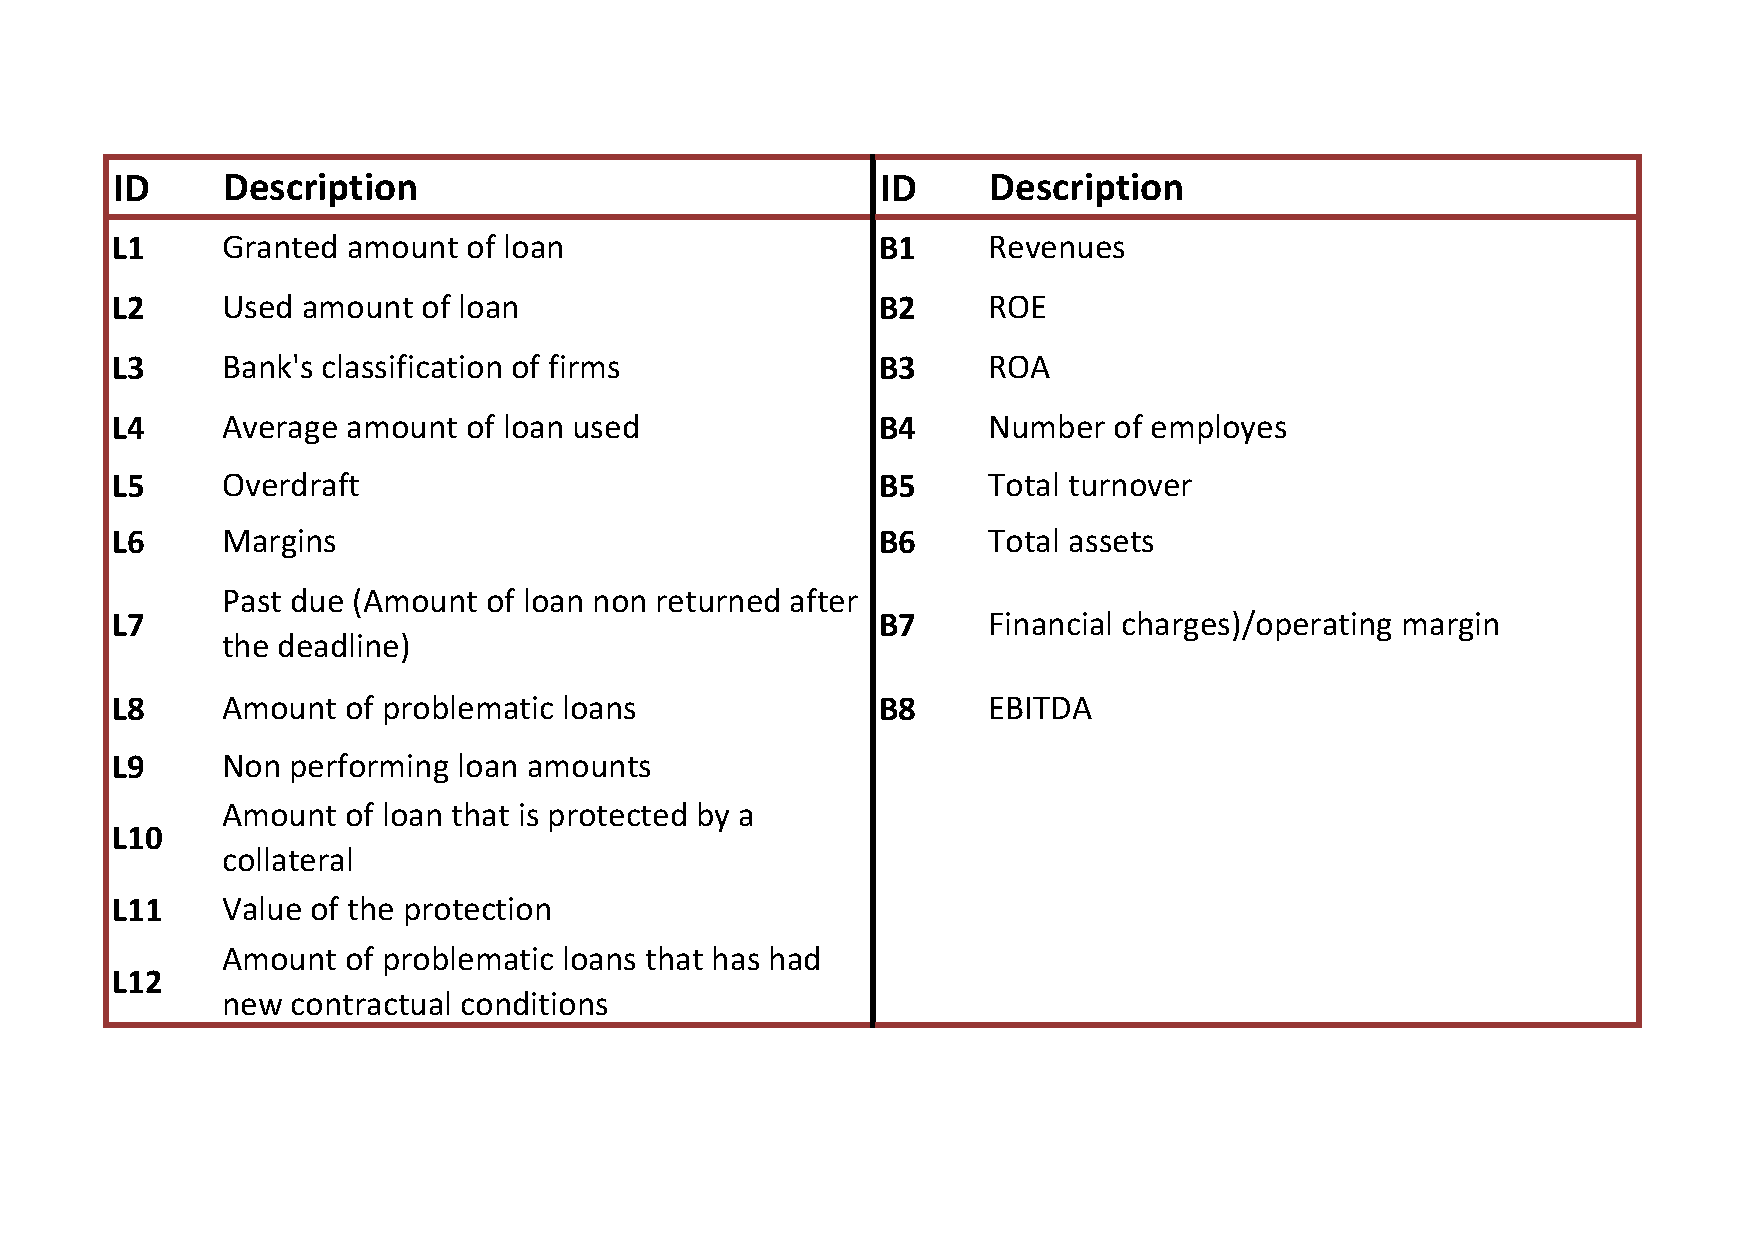
\includegraphics[width=180mm, height=80mm]{figs/Table_dataset.pdf}
%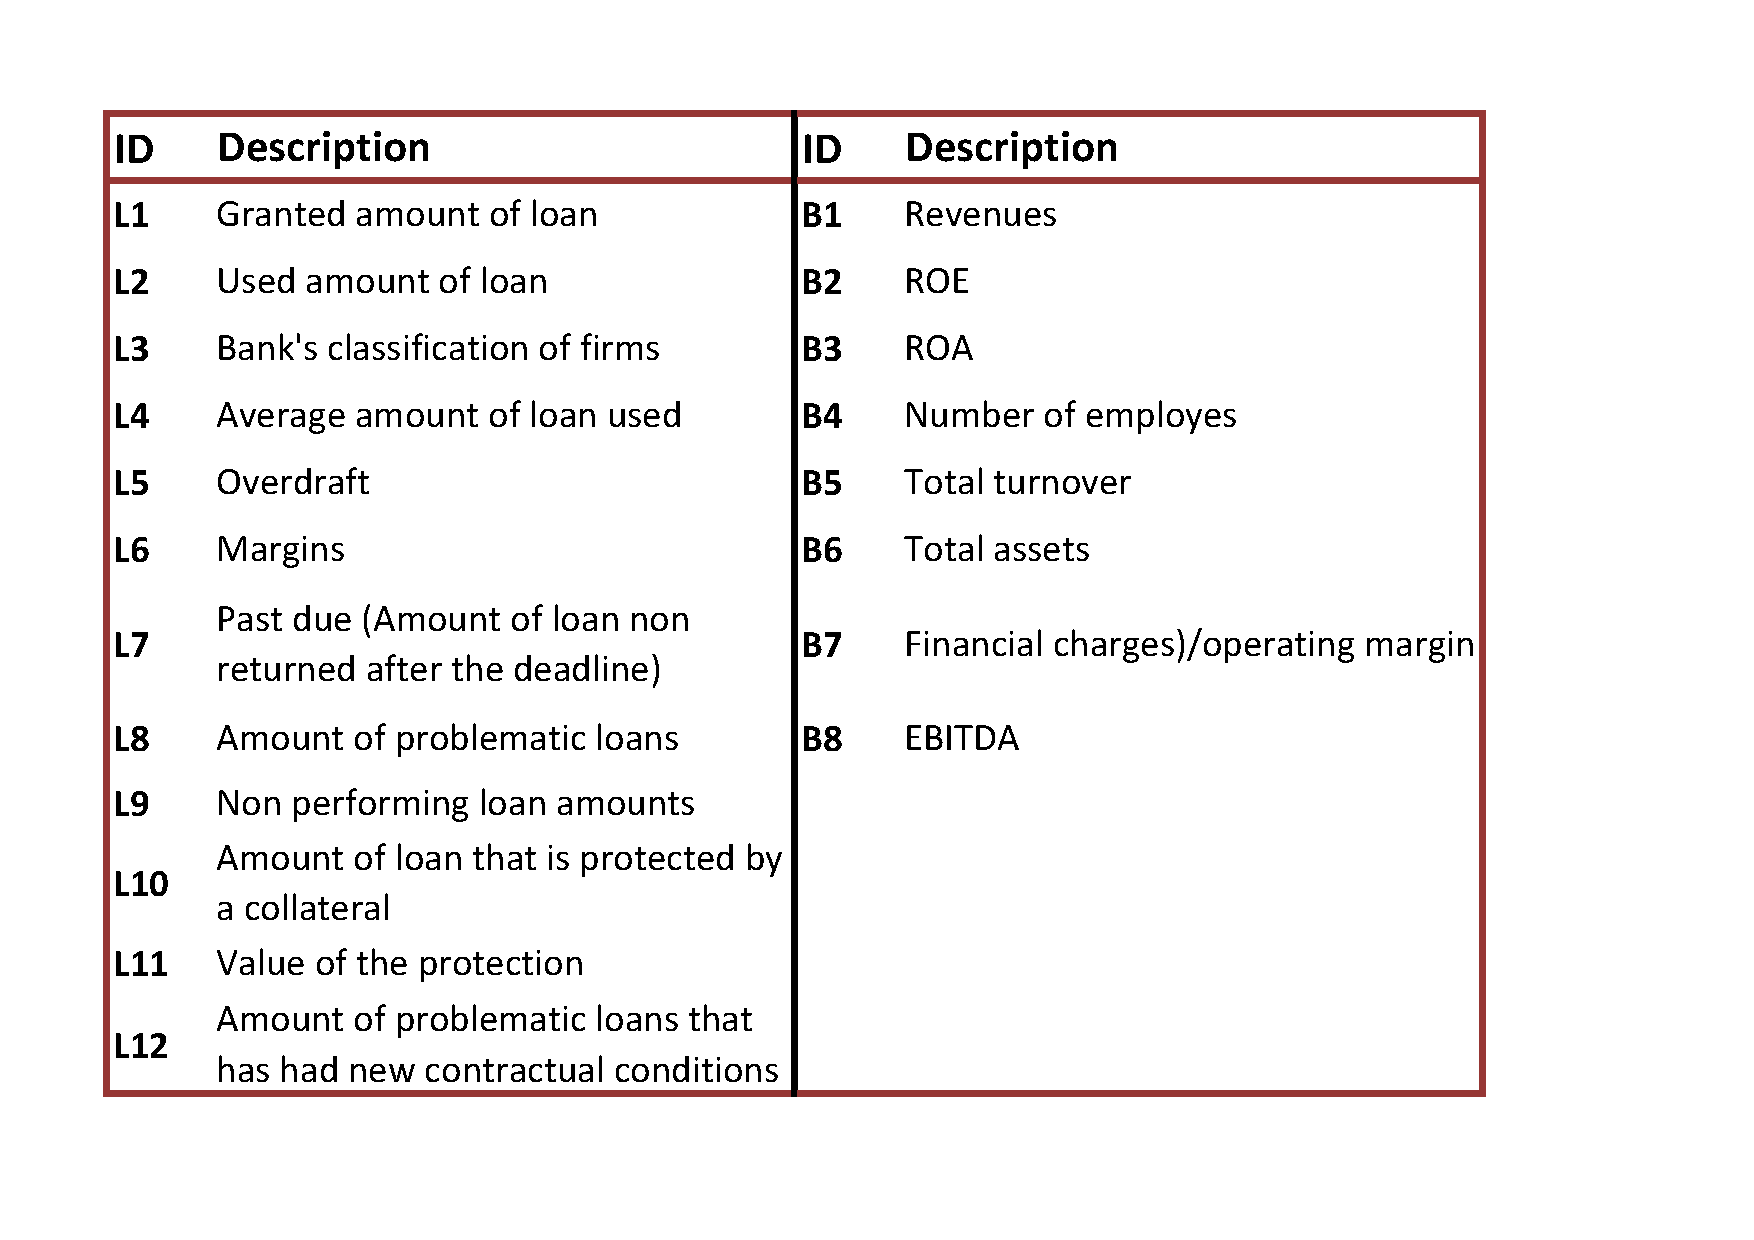
\includegraphics[width=180mm, height=80mm]{figs/Cdataset.pdf}
%\caption{Loan dataset (L) and Balance sheet dataset (B): main
%attributes. Loans data are quarterly from 2009 to 2014;
%Balance sheet data have annual frequency from 2006 to 2014}
%\end{figure}

\begin{table}
\small
\begin{center}
\begin{tabular}{ lllc | lllc }
\hline
& & & & & & &  \\
   &  \textbf{ID}       &\textbf{Description} &  & & \textbf{ID}       &\textbf{Description}   &\\
\hline
\hline
\\
&\textbf{C1}    &Granted amount of loans & & &\textbf{A1}  &Firm's default status (assessed by banks)   &  \\
&\textbf{C2}    &Used amount of loans & & &\textbf{A2}  &Loan expenses   &  \\
&\textbf{C3}    &Bank's classification of firm & & &\textbf{A3}  &Loan arrears   &  \\
&\textbf{C4}    &Average amount of loan used& & &\textbf{A4}  &Initial loan Commitment     & \\
&\textbf{C5}    &Overdraft & & &\textbf{A5}  &Outstanding nominal amount of loan    & \\
&\textbf{C6}    &Margins & & &\textbf{A6}  &Off-balance sheet amount     & \\
&\textbf{C7}    &Past due (loans not returned after the deadline) & & &\textbf{A7}  &Amount of protection   & \\
&\textbf{C8}    &Amount of problematic loans & & &\textbf{A8}  &Probability of default of firm (assessed by banks)  & \\
&\textbf{C9}    &Amount of non-performing loans & & &  &  & \\
&\textbf{C10}    &Amount of loans protected by a collateral & & &  &  & \\
&\textbf{C11}    &Value of the protection & & &  &  & \\
&\textbf{C12}    &Previous "Adjusted default" classification & & &  &  & \\
\hline
\\
\end{tabular}
\caption{Main attributes for the two credit datasets: Central Credit Register (C) and  AnaCredit (A)}
%The loan dataset contains credit data for about 800,000
%Italian firms and has quarterly frequency from 2009 to 2014. Balance
%sheet dataset contains data for about 300,000 Italian firms with
%annual frequency from 2006 to 2014. Companies for which balance
%sheet data are available represent a subset of the previous loan
%dataset consisting of the largest firms.
\label{tbl:attributes}
\end{center}
\end{table}


\begin{table}
\small
\begin{center}
\begin{tabular}{| lll | }
\hline

   &  \textbf{ID}       &\textbf{Description} \\
\hline
\hline
 &  \ & \\
&\textbf{X1}    &Revenues   \\
&\textbf{X2}    &Employees   \\
&\textbf{X3}    &Total added value  \\
&\textbf{X4}    &MOL \\
&\textbf{X5}    &Active  \\
&\textbf{X6}    &Working Capital  \\
&\textbf{X7}    &Net Equity \\
&\textbf{X8}    &ROE  \\
&\textbf{X9}    &ROI \\
&\textbf{X10}    &ROA   \\
&\textbf{X11}    & Margin on revenues \\
&\textbf{X12}    &Operating costs/production value  \\
&\textbf{X13}    &MOL/production value\\
&\textbf{X14}    &MOL/operational added value\\
&\textbf{X16}    &Liquidity\\
&\textbf{X17}    &Total equity/financial debt\\
&\textbf{X18}    &Bank financial debt+ICS/financial debt\\
&\textbf{X19}    &Financial expenses/MOL\\
&\textbf{X20}    &Ebitda/Net financial charges\\
&\textbf{X24}    &Current profit\\
&\textbf{X34}    &Net revenues/operating assets\\

\hline

\end{tabular}
\caption{Main attributes for the balance sheet dataset (X)
.}
\label{tbl:attributes}
\end{center}
\end{table}




\paragraph{The Balance-sheets dataset.}

Our second dataset consists of the balance-sheet data of about $300K$
Italian firms. They are generally medium and large companies and they
form a subset of the $800K$ companies with loan data. 
It contains balance-sheet information for years from 20013 and 2014.
The main features include those that regard the profitability of a company, such as return
of equity (ROE) and return of assets (ROA); see Table~\ref{tbl:attributes} for a more
extended list. Typically balance sheet data are public data and have been used extensively for
bankruptcy prediction (e.g., see Barboza et
al.~\cite{altman-bankruptcy-17} and references therein).

\paragraph{The AnaCredit dataset.}

The third dataset is a dataset with detailed information on individual bank loans in the euro area. The name of the dataset is “AnaCredit” and it stands for “analytical credit datasets”.
AnaCredit is a shared multipurpose database containing loan-by-loan information on credit extended by credit institutions to companies and other legal entities. On 18 May 2016 the Governing Council of the ECB adopted Regulation ECB/2016/13 on the collection of granular credit and credit risk data (AnaCredit) establishing Stage 1 of a shared database for the European System of Central Banks (ESCB) as of September 2018. The database will contain a large number of credit information, updated mostly on a monthly basis, based on harmonised concepts and definitions common to all participating countries.
AnaCredit is a shared multipurpose database that will contain loan-by-loan information on credit to companies and other legal entities extended by credit institutions and their foreign branches on a monthly basis. Based on compelling requests from   users in a large number of central banks’ business areas, AnaCredit data collection has been designed with a view to obtaining a complete picture of a) the total credit exposure of the European banks and b) the total indebtedness of borrowers across all lenders. The information collected consists of 88 different attributes based on harmonised concepts and definitions and covers various aspects of the credit exposure.

In the Table ~\ref{tbl:attributes} we can see the main features we will consider in the paper in order to try to predict firms bank default. 
This information also includes some important vulnerability indicators assessed by banks, such as default status and probability of default of companies that have relationships with banks.

\paragraph{Merged credit dataset.}

The AnaCredit dataset contains monthly information for approximately 800,000 Italian companies as of June 2018.
In order to predict bank failure we will use a combined dataset comprising data from the CCR and AnaCredit datasets. We will use data from the past two years (June 2018 to June 2020) to try to predict companies that were in a "good situation" with respect to the Italian banking system in June 2019 and that will result in Adjusted bank default in June 2020. The overall dataset we will use contains over 570,000 companies for a total of 136 features.






\begin{comment}
    

Our second dataset consists of the balance-sheet data of about $300K$
Italian firms. They are generally medium and large companies and they
form a subset of the $800K$ companies with loan data. 
It contains balance-sheet information for each year from 2006 to 2014.
The main features include those that regard the profitability of a company, such as return
of equity (ROE) and return of assets (ROA); see Table~\ref{tbl:attributes} for a more
extended list. Typically balance sheet data are public data and have been used extensively for
bankruptcy prediction (e.g., see Barboza et
al.~\cite{altman-bankruptcy-17} and references therein).
%
%Among the
%fundamental ones are those regarding the profitability of companies, as
%in the case of ROE and ROA.
%
%
%With the aim of improving the forecasts of the default status of Italian
%firms, we have also performed some classification attempts  by
%integrating credit information with some balance sheet indicator for Italian
%companies. In particular, we used a set of firms balance sheet
%indicators from the CEBI dataset: some important indicators are used
%that are very similar to those used by Barboza et al.
%\cite{altman-bankruptcy-17} also  in his famous Z-score. Among the
%fundamental ones are those regarding the profitability of companies, as
%in the case of ROE and ROA. The balance sheet dataset contains data
%related to about 300,000 Italian firms; these are generally medium and
%large companies. For each firms we used a set of eight indicators shown
%in the Table. Balance sheet data are public data.\\
%
%The three hundred thousand companies for which balance sheet data are
%available constitute a sub-sample of those belonging to the loan
%dataset. Therefore the dataset that uses both information on loans and
%balance sheet info is made up of about 300,000 companies.

\end{comment}

\paragraph{Heavy imbalanced dataset}

A lot of modern problems in the machine learning field have to deal with imbalanced datasets. For some of them, the problem is due to the lack of data samples, for others to the intrinsic nature of the problem.
While for the first group it’s easier to find a way around the problem for the second it represents a characteristic of the dataset itself and would make the prediction capability of any model much lower. 
In this case, the problem falls into the second category since we are trying to assess the likelihood of companies to fail and just a small amount of the total fail over the year. For our dataset described above, the ratio between failed and healthy companies is close to 2%.

\subsection{Evaluation criteria}
We use a variety of evaluation measures to assess the effectiveness of
our classifiers, which we briefly define. As usually, in a binary
classification context, we use the standard concepts of true positive
(TP), false positive (FP), true negative (TN), false negative (FN):
\medskip

\begin{center}
\begin{tabular}{|l|c|c|}
\hline
	& Predicted Default	& Predicted Not Default \\\hline
Default 	&\TP	&\FN	\\\hline
Did not default &\FP	&\TN	\\\hline
\end{tabular}
\end{center}
\medskip

For instance, FN is the number of firms that defaulted during a particular year but
the classifier predicted that they will not default.


We now define the measures that we use:
\begin{itemize}
\item Precision: $\displaystyle \Precision=\frac{\TP}{\TP+\FP}$
\item Recall: $\displaystyle \Recall=\frac{\TP}{\TP+\FN}$
\item F1-score: $\displaystyle \FOne=2\cdot\frac{\Precision\cdot\Recall}{\Precision+\Recall}$
%\item Type-I Error: $\displaystyle \TypeOne=\frac{\FN}{\TP+\FN}$
%\item Type-II Error: $\displaystyle \TypeTwo=\frac{\FP}{\TN+\FP}$
%\item Balanced Accuracy: $\Bacc \FOne=2\cdot\frac{\TP\cdot\TN}{\TP+\TN}$
% \item Mattews correlation coefficient: \textbf{MCC}
% \item  \textbf{Kappa}
\item Area under the ROC curve: \textbf{AuROC}
\item True positive rate: \textbf{TPR}
\item True negative rate: \textbf{TNR}
\end{itemize}

Our analysis of the results will be particularly focused on considering the AuROC, which is a particularly useful indicator for performance comparisons as it is widely used in literature.


